\documentclass[a4paper,12pt,landscape,twocolumn]{article}
\usepackage{wordlike}
\usepackage[UKenglish]{isodate}
\usepackage{graphicx}
\usepackage{multicol}

\raggedright
\setlength{\parskip}{1ex}

\newcommand{\documenttitle}{Shropshire Botanical Society Online Flora}
\newcommand{\documentauthor}{Joe J Collins}

\title{Shropshire Botanical Society Online Flora\\
Web application Specification}
\author{\documentauthor}
\date{\today}

\usepackage[pdftex,
  pdftitle={\documenttitle}, 
  pdfauthor={\documentauthor},
  pdfsubject={\documenttitle}]{hyperref}

\begin{document}
\maketitle
\tableofcontents
\vfil
\pagebreak
\section{Summary}

The Shropshire Botanical Society seeks to provide access to 
collected records
\clearpage

\section{Background}

The Shropshire Botanical Society
(referred to here as `the Society')
has been dedicated to promoting the enjoyment,
understanding and conservation of the flora of Shropshire
since XXX.
One of the principle activities of the Society is to collect and maintain records 
of plant sightings within the historical boundaries of the county of Shropshire.
The Society has a database of records dating as far back as the 18\textsuperscript{th} century.
Since 2003 the Society has made these records freely available online via a bespoke web application
or Online Flora.
The web application is still available at 
\href{https://captain-blue.azurewebsites.net/}{https://captain-blue.azurewebsites.net/}
but unfortunately the data is now many years out of date.
This original Online Flora was written using
PHP and \href{https://codeigniter.com/}{CodeIgniter Web Framework}
backed by MySql database.

Currently all the Society's records are also submitted to the 
\href{https://nbnatlas.org/}{National Biodiversity Network Atlas}
and 2017 the Society's records have been available via a web service at
\href{https://api.nbnatlas.org/}{https://api.nbnatlas.org/}.

The Society now seeks to build on the success of their earlier Online Flora,
by revising the web application
to make use of National Biodiversity Network Atlas web service to provide the data,
whilst also providing a more modern mobile interface.

\section{Searching and Scenarios}

Search only, no data entry,

The new web application should largely replicate the functionality of the original web application.
It should therefore provide a method to search for

\begin{description}
    \item[Name] records of a sep
    \item[Site]
    \item[Monad or Grid Square] or   
\end{description}

\section{Users}

Knowledgeable
In the field on mobile (Android)
Home research on desktop (the majority of Window and Chrome)


\clearpage
\section{Search County by Plant Name}
\subsection{Mobile}
\begin{multicols}{1}
    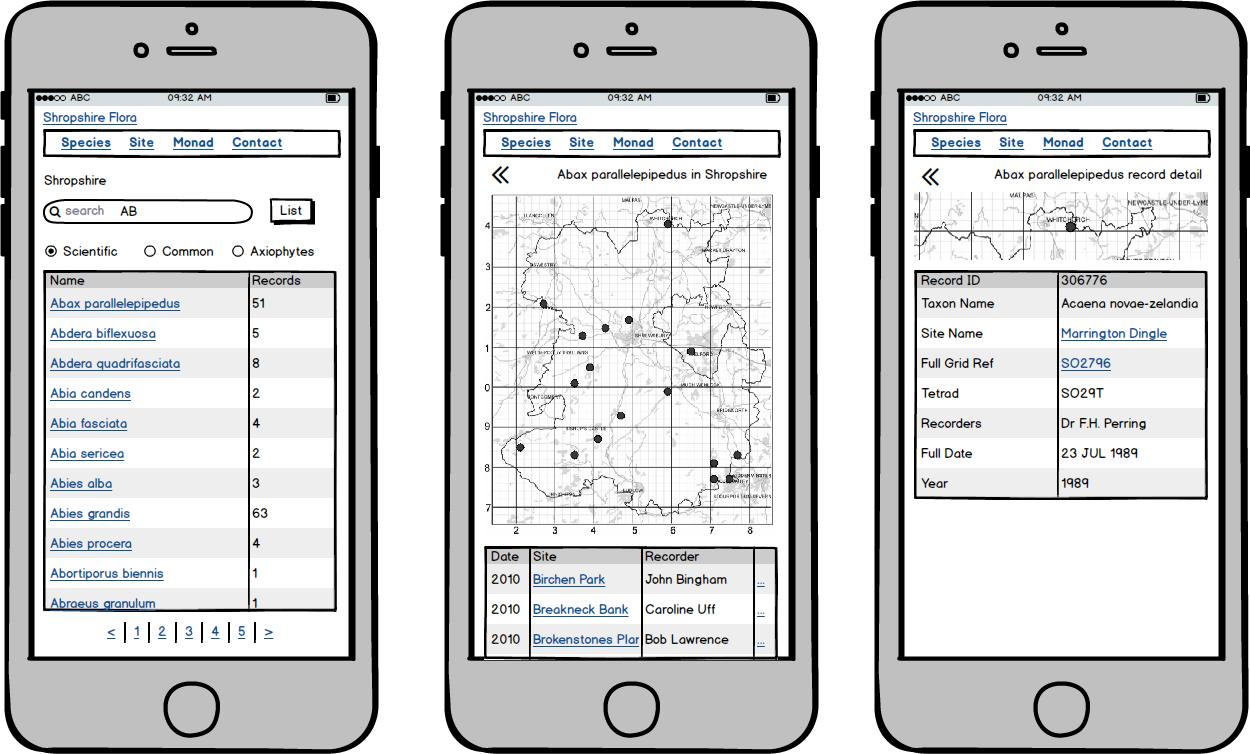
\includegraphics[width=0.9\textwidth]{./wireframes/county-mobile.png}
\end{multicols}

Search within the entire collection for the county.

\begin{description}
    \item[Scientific Name] selected by default.
    \item[Common Name] where common name is selected only those sightings with a common name will be show.
    \item[Axiophytes] 
\end{description}


\clearpage
\subsection{Desktop}
\begin{multicols}{1}
    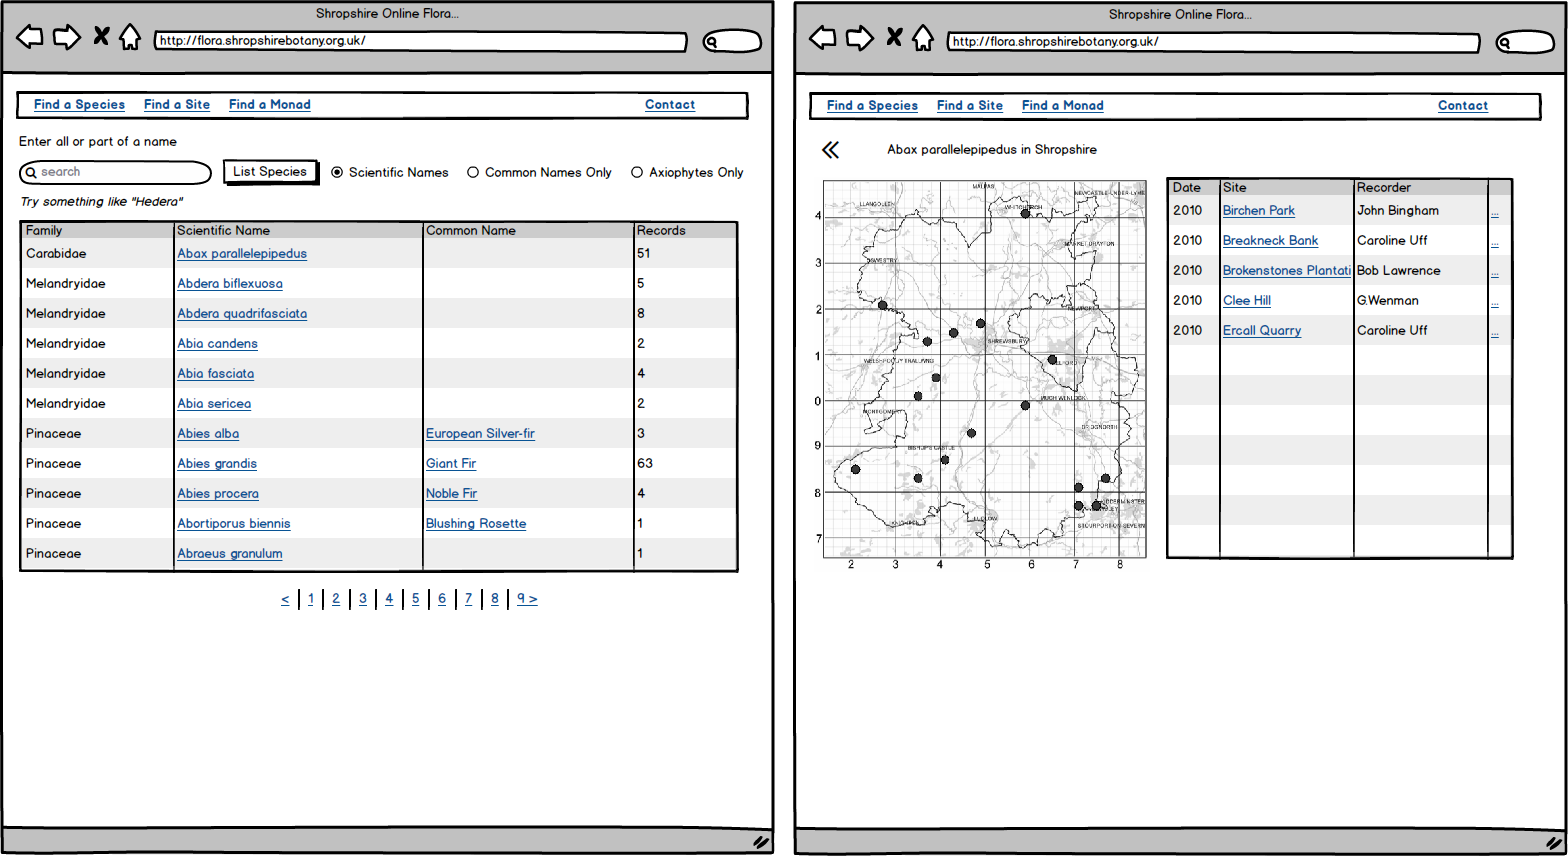
\includegraphics[width=0.6\textwidth]{./wireframes/county-desktop.png}
\end{multicols}



\clearpage
\section{Search Grid Square by Plant Name}
\subsection{Mobile}
\begin{multicols}{1}
    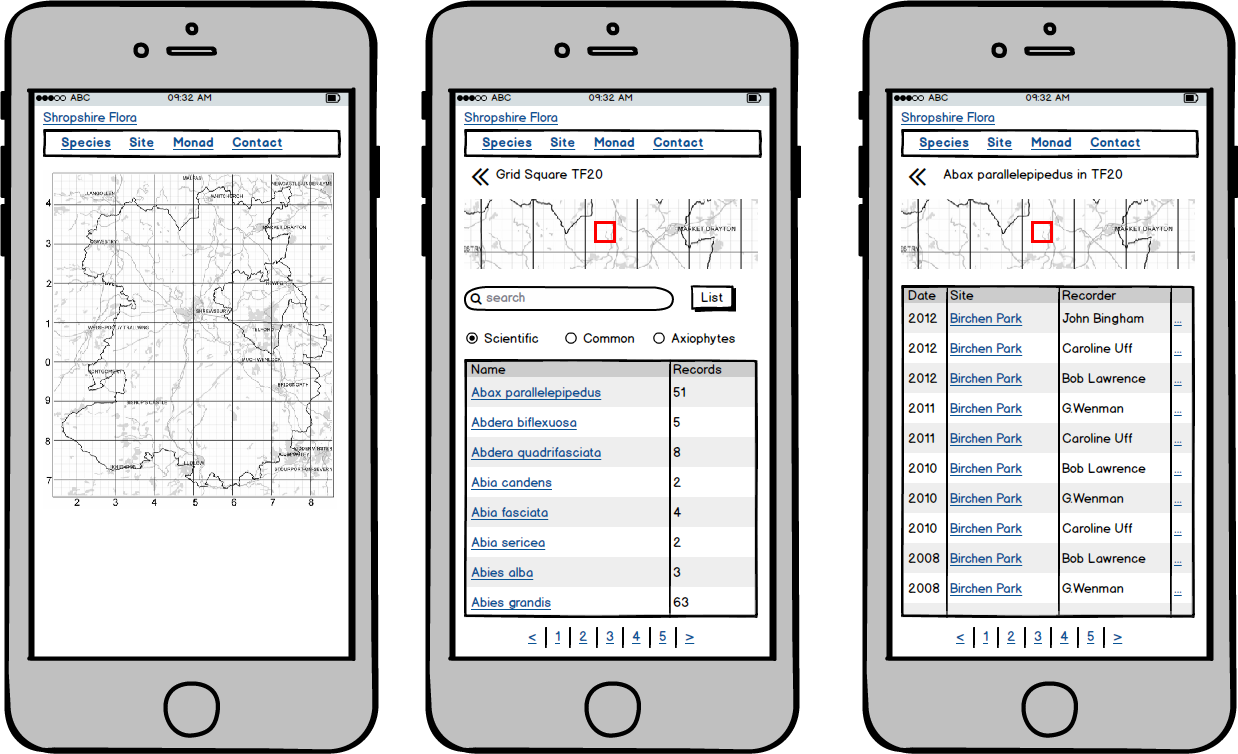
\includegraphics[width=0.9\textwidth]{./wireframes/monad-mobile.png}
\end{multicols}


\section{Technical Constraints}

Success with PHP and CodeIgniter
Happy with PHP source developers from within the ranks of members.

\begin{description}
    \item[PHP 7.3] for deployment to Google App Engine.
    \item[CodeIgniter 4.0.4] happ with 
        No Caching to reveal performance, caching later.
    \item[Twitter Bootstrap 4.5.2] for responsive.
        No Client Detection Just responsive.
    \item[Leaflet 1.6.0] Mapping https://github.com/DuncanRowland/NBNMapOverlayExamples
    \item[No NBN API Calls from the Client] 
    \item[Commits to Github] branching but no where else.
        at \href{https://github.com/joejcollins/captain-magenta.git}{Github}
      The Society will
    \item[Style Sheet] from the Website
    \item[JavaScript] plain 
    \item[Google Analytics] embed.
\end{description}

\end{document}


